\documentclass[9pt,a4paper,twocolumn]{article}
\usepackage[utf8]{inputenc}
\usepackage[T1]{fontenc}
\usepackage[brazilian]{babel}
\usepackage[margin=1.4cm,columnsep=0.6cm]{geometry}
\usepackage{booktabs}
\usepackage{graphicx}
\usepackage{amsmath}
\usepackage{xcolor}
\usepackage[font=small,labelfont=bf,skip=3pt]{caption}
\usepackage[expansion=false]{microtype}
\usepackage[hidelinks]{hyperref}
\usepackage{titlesec}
\usepackage{enumitem}
\usepackage{multirow}
\usepackage{float}
\usepackage{indentfirst}
\usepackage{placeins}

\setlength{\parskip}{2pt}
\setlist{nosep,leftmargin=1.2em}
\titlespacing*{\section}{0pt}{8pt}{3pt}
\titlespacing*{\subsection}{0pt}{5pt}{2pt}
\renewcommand{\arraystretch}{1.05}

% Em modo twocolumn a coluna tem ~8.7cm de largura.
\setlength{\textfloatsep}{6pt plus 2pt minus 2pt}
\setlength{\floatsep}{6pt plus 2pt minus 2pt}
\setlength{\intextsep}{6pt plus 2pt minus 2pt}
\setlength{\abovedisplayskip}{3pt plus 1pt minus 1pt}
\setlength{\belowdisplayskip}{3pt plus 1pt minus 1pt}

\renewcommand{\floatpagefraction}{0.7}
\renewcommand{\dblfloatpagefraction}{0.7}
\renewcommand{\textfraction}{0.1}
\renewcommand{\topfraction}{0.9}
\renewcommand{\dbltopfraction}{0.9}
\renewcommand{\bottomfraction}{0.65}

\newcommand{\bmk}{\textsc{BM25}}
\newcommand{\rrf}{\textsc{RRF}}
\newcommand{\ndcg}{\textsc{NDCG}}
\newcommand{\map}{\textsc{MAP}}

\graphicspath{{figures/}}

\title{\vspace{-1.2cm}\textbf{Trabalho Prático 2}\vspace{-0.2cm}}
\author{
Gustavo Cardozo de Moraes Moreira \\
NUSP: 5244057; Email: gucmm@usp.br; Filiação: ICMC-USP\\
Matheus Rodrigues Ferreira\\
NUSP: 14762149; Email: matheus.rf@usp.br; Filiação: ICMC-USP
}

\begin{document}
\maketitle
\vspace{-0.6cm}

%------------------------------------------------------------------------------
\section{Introdução}
Sistemas modernos de Recuperação de Informação combinam evidências de naturezas distintas: a
busca lexical, que casa termos da consulta com os do documento, e a busca semântica, que projeta
textos em um espaço vetorial denso capaz de aproximar expressões de significado equivalente.
Sobre os rankings desses dois sistemas, aplicam-se mecanismos de fusão (busca híbrida),
reranking neural e, em aplicações generativas, a seleção de contexto e a geração de respostas
por um modelo de linguagem (Retrieval-Augmented Generation, RAG).

O objetivo deste trabalho é desenvolver e avaliar, de forma quantitativa e reprodutível, um
pipeline completo de recuperação sobre a coleção \textsc{NFCorpus} (benchmark BEIR):
pré-processamento e indexação, recuperação lexical (\bmk{}) e semântica (bi-encoder), fusão por
\textit{Reciprocal Rank Fusion} (\rrf{}), reranking com \textit{cross-encoder} e RAG com um
modelo aberto (Qwen). Além de medir qual combinação atinge o melhor desempenho, investigamos,
com evidências extraídas dos próprios experimentos, \emph{por que} os sistemas diferem em
consultas específicas e onde o pipeline falha ponta a ponta.

O estudo é guiado pelas seguintes perguntas:
\begin{itemize}
  \item Qual sistema é melhor em média --- lexical ou semântico --- e em quais consultas a ordem se inverte?
  \item Quanto do desempenho perdido por erros de digitação é recuperado pela correção ortográfica (k-gramas + Jaccard + distância de edição)?
  \item A fusão híbrida (\rrf{}) e o reranking (cross-encoder) melhoram as métricas do recuperador inicial?
  \item Como o RAG afeta a fidelidade, a completude, a utilidade e a rastreabilidade das respostas geradas?
  \item Em que estágio (recuperação, fusão, reranking, seleção de contexto ou geração) ocorrem as falhas ponta a ponta?
\end{itemize}

Todos os experimentos usam a mesma coleção, as mesmas consultas e os mesmos julgamentos
(qrels); os qrels são empregados exclusivamente na avaliação, e o conjunto \emph{test} foi
reservado para a avaliação final, usando-se apenas o \emph{dev} para ajuste de parâmetros.

%------------------------------------------------------------------------------
\section{Metodologia}
O pipeline foi implementado em Python 3.14, com \texttt{nltk} (stopwords e stemming),
\texttt{sentence-transformers} (bi-encoder e cross-encoder), \texttt{transformers}/\texttt{torch}
(LLM), \texttt{numpy} e \texttt{pandas}. O índice invertido foi implementado do zero. Todos os
componentes ficam em módulos reutilizados por todos os experimentos, garantindo o mesmo
pré-processamento e as mesmas consultas em todas as comparações.

\subsection{Pré-processamento}
Documentos e consultas passam pelo mesmo pipeline, em ordem: (1) conversão para minúsculas;
(2) remoção de pontuação por expressão regular, mantendo apenas letras, dígitos e espaços;
(3) tokenização por espaço; (4) remoção de \emph{stopwords} do inglês (NLTK); (5) \emph{stemming}
com o algoritmo de Porter (NLTK). Os campos \texttt{title} e \texttt{text} de cada documento são
concatenados para formar a representação usada em todos os sistemas, conforme exigido pelo
enunciado.

\subsection{Índice invertido}
O índice foi construído do zero usando apenas dicionários nativos do Python: um dicionário
termo $\rightarrow$ \emph{posting list} (por sua vez um dicionário \texttt{doc\_id} $\rightarrow$
frequência do termo, $\mathrm{tf}$), além das estruturas com a frequência documental
($\mathrm{df}$), o comprimento de cada documento e as estatísticas globais ($N$, total de tokens,
comprimento médio). Essas são exatamente as informações exigidas pelo \bmk{}, e a consulta
acessa apenas as \emph{posting lists} dos termos presentes na consulta --- nunca a coleção
inteira. O índice registra $18\,929$ termos de vocabulário, $359\,991$ postings e é construído em
$0{,}27$~s.

\subsection{Busca lexical (\bmk{})}
A função de escore é
\[
\mathrm{score}(q,d)=\sum_{t\in q} \mathrm{IDF}_t \cdot
\frac{\mathrm{tf}_{t,d}\,(k_1+1)}{\mathrm{tf}_{t,d}+k_1\big(1-b+b\,\tfrac{|d|}{\mathrm{avgdl}}\big)},
\]
com $\mathrm{IDF}_t=\ln\!\big((N-\mathrm{df}_t+0{,}5)/(\mathrm{df}_t+0{,}5)+1\big)$ e os valores
padrão $k_1=1{,}5$ e $b=0{,}75$. O \bmk{} foi escolhido como baseline lexical por ser o modelo
probabilístico de referência, com saturação da frequência do termo ($k_1$) e normalização pelo
comprimento ($b$).

\subsection{Tolerância a erros}
A correção ortográfica segue o protocolo do enunciado, em três passos: (1) geração de candidatos
por k-gramas de caracteres (trigramas com padding nas bordas), usando um índice invertido de
k-gramas $\rightarrow$ termos; (2) filtragem pelo coeficiente de Jaccard entre os conjuntos de
k-gramas (limiar $0{,}2$); (3) seleção por distância de edição com suporte a transposição
(Damerau--Levenshtein, custo máximo $3$), desempatando pelo termo mais frequente (DF). O
dicionário é formado pelos termos da coleção \emph{antes} do stemming, sem stopwords.

\subsection{Recuperação semântica}
Usamos o bi-encoder \texttt{sentence-transformers/all-MiniLM-L6-v2} (384 dimensões), que gera
embeddings normalizados; a similaridade é o cosseno (produto interno dos vetores unitários). Os
embeddings dos documentos são calculados uma única vez e armazenados em disco; para cada consulta
calcula-se o embedding e a similaridade com todos os documentos (busca exaustiva, permitida pela
coleção pequena). O comprimento máximo de entrada é 256 tokens, com truncamento.

\subsection{Busca híbrida (\rrf{})}
Os rankings lexical e semântico (top-100 de cada) são fundidos por \textit{Reciprocal Rank Fusion}:
\[
\mathrm{RRF}(d)=\sum_{s}\frac{1}{k+\mathrm{rank}_s(d)},
\]
em que $\mathrm{rank}_s(d)$ é a posição de $d$ (a partir de 1) no sistema $s$; documentos ausentes
de um ranking não recebem contribuição daquele sistema. O parâmetro $k$ foi ajustado no conjunto
\emph{dev} entre $\{10,60,100\}$.

\subsection{Reranking}
Os 50 primeiros documentos do ranking híbrido são reordenados por um \textit{cross-encoder}
pré-treinado (\texttt{cross-encoder/ms-marco-MiniLM-L6-v2}), que pontua o par
(consulta, documento) conjuntamente. Os documentos abaixo da posição 50 mantêm a ordem relativa do
ranking híbrido, preservando um ranking completo. O comprimento máximo de entrada é 512 tokens,
com truncamento.

\subsection{RAG}
O pipeline de geração é consulta $\rightarrow$ híbrido $\rightarrow$ reranking $\rightarrow$
seleção do Top-5 $\rightarrow$ LLM $\rightarrow$ resposta. Cada item do corpus é uma unidade de
contexto. A LLM é o \texttt{Qwen/Qwen2.5-1.5B-Instruct}, executada localmente via
\texttt{transformers} (float16), com temperatura $0$, seed $42$ e máximo de 512 tokens, gerando em
português (sem custo de API; hardware na Seção~\ref{avaliacao}). Foram executadas duas condições com os mesmos parâmetros: (A) sem RAG, em que a LLM
recebe apenas a pergunta; e (B) com RAG, em que recebe a pergunta e os Top-5 documentos com seus
\texttt{doc\_id}s, instruída a responder com base no contexto, indicar as fontes e informar quando
não houver evidência suficiente.

%------------------------------------------------------------------------------
\section{Avaliação}\label{avaliacao}

\textbf{Conjunto de dados.} \textsc{NFCorpus} (BEIR): $3\,633$ documentos médicos (título +
texto), $3\,237$ consultas e julgamentos em \texttt{qrels/dev.tsv} (324 consultas) e
\texttt{qrels/test.tsv} (323 consultas). O \emph{dev} foi usado apenas para ajuste de parâmetros;
o \emph{test}, reservado para a avaliação final.

\textbf{Relevância.} Para as métricas binárias (P, R e AP), é relevante todo documento com grau de
relevância $>0$. Para o \ndcg{}, os graus fornecidos pelos qrels são preservados.

\textbf{Métricas.} Seja $R_q$ o conjunto de relevantes de $q$ e $\mathrm{Top}_k$ os $k$ primeiros
do ranking. Com $k=10$, calculamos por consulta:
\[
\mathrm{P@}k=\frac{|\mathrm{Top}_k\cap R_q|}{k};\qquad
\mathrm{R@}k=\frac{|\mathrm{Top}_k\cap R_q|}{|R_q|},
\]
\[
\mathrm{AP@}10=\frac{1}{|R_q|}\sum_{\substack{i\le 10\\ d_i\in R_q}}\mathrm{P@}i,\qquad
\mathrm{MAP@}10=\frac{1}{|Q|}\sum_{q\in Q}\mathrm{AP@}10(q),
\]
com a convenção do \texttt{trec\_eval} (denominador $=|R_q|$, e não o mínimo com $k$). O \ndcg{}
usa ganho linear (ganho $=$ grau de relevância):
\[
\mathrm{DCG@}k=\sum_{i=1}^{k}\frac{\mathrm{rel}_i}{\log_2(i+1)},\qquad
\mathrm{NDCG@}k=\frac{\mathrm{DCG@}k}{\mathrm{IDCG@}k},
\]
com o $\mathrm{IDCG}$ calculado a partir de \emph{todos} os julgamentos da consulta, não apenas
dos documentos recuperados. As médias globais e os valores por consulta estão em
\texttt{outputs/}.

\textbf{Ambiente computacional.} Windows 10, Python 3.14, PyTorch 2.12 (CPU), 7,4~GB de RAM.
Protocolo reproduzível com sementes fixas (seed 42 na seleção das consultas do RAG e na
geração da LLM).

%------------------------------------------------------------------------------
\section{Resultados Obtidos e Análise}

\subsection{Índice e busca lexical $\times$ semântica}

\begin{table}[h]
\centering
\small
\begin{tabular}{lcccc}
\toprule
Sistema & P@10 & R@10 & MAP@10 & NDCG@10\\
\midrule
Lexical (\bmk{}) & 0{,}2412 & 0{,}1551 & 0{,}1225 & 0{,}3302\\
Semântico & 0{,}2433 & 0{,}1550 & 0{,}1105 & 0{,}3160\\
Híbrido (\rrf{}, $k{=}10$) & \textbf{0{,}2601} & \textbf{0{,}1740} & 0{,}1365 & \textbf{0{,}3562}\\
Híbrido + reranking & 0{,}2508 & 0{,}1674 & \textbf{0{,}1388} & 0{,}3562\\
\bottomrule
\end{tabular}
\caption{Métricas médias no conjunto \emph{test} (corte 10).}
\label{tab:metricas}
\end{table}

\begin{figure}[h]
    \centering
    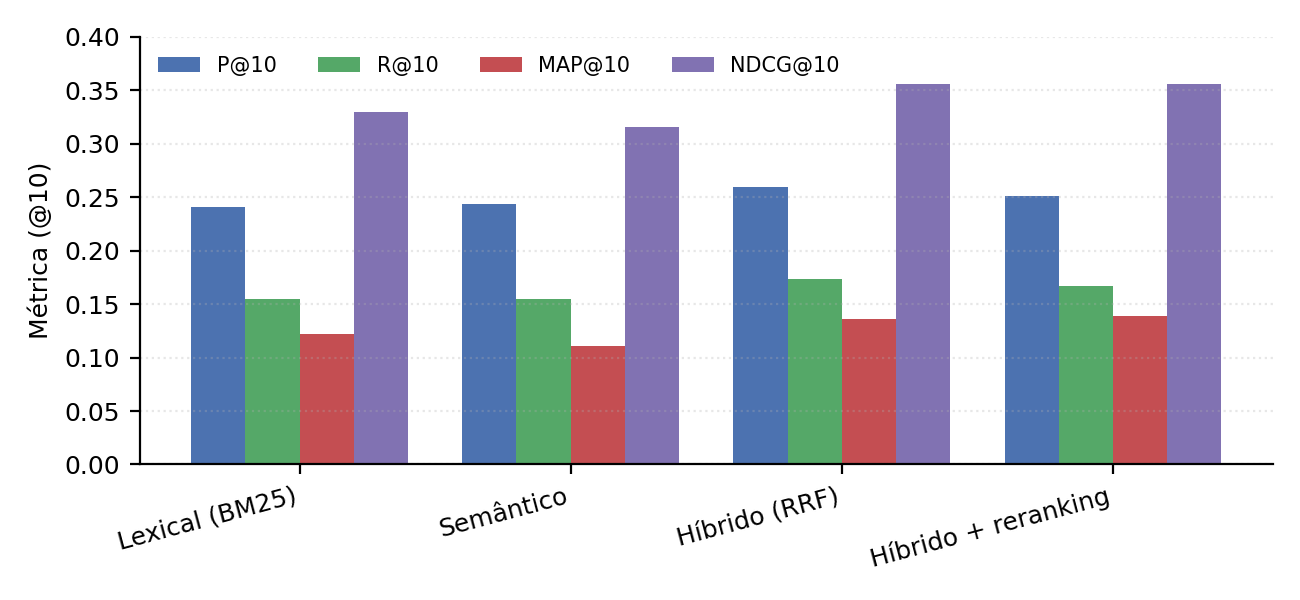
\includegraphics[width=\linewidth]{fig_metricas.png}
    \caption{Métricas médias dos quatro sistemas no conjunto \emph{test}.}
    \label{fig:metricas}
\end{figure}

A Tabela~\ref{tab:metricas} e a Figura~\ref{fig:metricas} mostram que o \bmk{} ($\ndcg{}@10=0{,}3302$) e o bi-encoder
($\ndcg{}@10=0{,}3160$) têm desempenho global próximo, com o lexical ligeiramente superior em
$\ndcg{}$ e $\map{}$, e o semântico com precisão marginalmente maior. A proximidade das médias,
porém, esconde diferenças grandes por consulta, exploradas a seguir.

\subsubsection{Análise por consulta}
Usando a diferença de $\ndcg{}@10$ por consulta, identificamos as três maiores vantagens de cada
sistema. O semântico vence em consultas em que o significado importa mais que o casamento exato de
termos. Em \texttt{PLAIN-924} (\emph{cocaine}), o \bmk{} retorna um único documento (MED-3044,
relevante), pois o termo aparece pouquíssimas vezes na coleção; o bi-encoder recupera, além dele,
MED-3054, MED-3055 e MED-3052 --- todos relevantes --- por capturar a similaridade temática entre
estudos sobre cocaína mesmo com vocabulário variado. Em \texttt{PLAIN-1537} (\emph{low-carb
diets}), o semântico posiciona quatro relevantes no Top-5, enquanto o lexical acerta apenas um.
Já em \texttt{PLAIN-3085} (\emph{The Difficulty of Arriving at a Vitamin D Recommendation}), a
consulta é longa e o lexical casa termos de alto IDF em contexto errado, enquanto o bi-encoder
recupera documentos sobre recomendações de vitamina D.

A vantagem do lexical aparece em consultas com termos técnicos raros, onde o casamento exato é
decisivo e o bi-encoder não distingue o conceito. Em \texttt{PLAIN-1473} (\emph{kohlrabi}), o
\bmk{} retorna exatamente o documento relevante (MED-4455); o bi-encoder retorna apenas
irrelevantes, pois ``kohlrabi'' é um termo raríssimo cujo embedding se aproxima de vegetais não
relacionados. O mesmo padrão ocorre em \texttt{PLAIN-2081} (\emph{shelf life}) e
\texttt{PLAIN-1288} (\emph{grapes}): o lexical concentra relevantes no Top-5, o semântico não
acerta nenhum. Em síntese, o bi-encoder é robusto a variação de vocabulário e sinonímia, mas se
perde em termos técnicos de baixa frequência, exatamente onde o casamento lexical é forte.

\begin{table}[h]
\centering
\scriptsize
\begin{tabular}{@{}p{1.15cm}p{7.0cm}@{}}
\toprule
\multicolumn{2}{@{}l}{\textit{Maior vantagem do semântico}}\\
\midrule
\multicolumn{2}{@{}l}{\textbf{PLAIN-3085} ``Vitamin D Recommendation'' ($\Delta\ndcg{}=+0{,}571$)}\\
Lexical & 3632\,(0; 11{,}42) · 2765\,(0; 10{,}24) · 919\,(0; 10{,}17) · 4872\,(0; 9{,}95) · 4575\,(0; 9{,}30)\\
Semânt. & 714\,(0; 0{,}70) · 4566\,(0; 0{,}64) · \textbf{4573\,(2; 0{,}64)} · \textbf{4570\,(2; 0{,}62)} · 919\,(0; 0{,}61)\\
\multicolumn{2}{@{}l}{\textbf{PLAIN-1537} ``low-carb diets'' ($\Delta\ndcg{}=+0{,}567$)}\\
Lexical & 4880\,(0; 22{,}51) · 2943\,(0; 6{,}33) · 1714\,(0; 6{,}22) · \textbf{4515\,(1; 6{,}02)} · 2458\,(0; 6{,}01)\\
Semânt. & \textbf{4515\,(1; 0{,}66)} · 4880\,(0; 0{,}61) · \textbf{4514\,(1; 0{,}60)} · \textbf{1616\,(1; 0{,}59)} · \textbf{2586\,(1; 0{,}56)}\\
\multicolumn{2}{@{}l}{\textbf{PLAIN-924} ``cocaine'' ($\Delta\ndcg{}=+0{,}558$)}\\
Lexical & \textbf{3044\,(1; 17{,}46)}\\
Semânt. & \textbf{3044\,(1; 0{,}47)} · \textbf{3054\,(1; 0{,}38)} · \textbf{3055\,(1; 0{,}34)} · \textbf{3052\,(1; 0{,}33)} · 4790\,(0; 0{,}31)\\
\midrule
\multicolumn{2}{@{}l}{\textit{Maior vantagem do lexical}}\\
\midrule
\multicolumn{2}{@{}l}{\textbf{PLAIN-1473} ``kohlrabi'' ($\Delta\ndcg{}=-1{,}000$)}\\
Lexical & \textbf{4455\,(1; 12{,}27)}\\
Semânt. & 3947\,(0; 0{,}22) · 4660\,(0; 0{,}22) · 3441\,(0; 0{,}22) · 3447\,(0; 0{,}21) · 5024\,(0; 0{,}21)\\
\multicolumn{2}{@{}l}{\textbf{PLAIN-2081} ``shelf life'' ($\Delta\ndcg{}=-1{,}000$)}\\
Lexical & \textbf{4303\,(1; 15{,}72)} · 1182\,(0; 12{,}20) · 2700\,(0; 11{,}19) · 2671\,(0; 10{,}73) · 2074\,(0; 8{,}69)\\
Semânt. & 1378\,(0; 0{,}42) · 2422\,(0; 0{,}39) · 2510\,(0; 0{,}39) · 4715\,(0; 0{,}38) · 1433\,(0; 0{,}37)\\
\multicolumn{2}{@{}l}{\textbf{PLAIN-1288} ``grapes'' ($\Delta\ndcg{}=-0{,}760$)}\\
Lexical & \textbf{2668\,(1; 10{,}39)} · \textbf{2669\,(1; 10{,}10)} · 2083\,(0; 9{,}78) · \textbf{1538\,(1; 9{,}78)} · \textbf{5065\,(1; 9{,}50)}\\
Semânt. & 3200\,(0; 0{,}43) · 3207\,(0; 0{,}43) · 398\,(0; 0{,}43) · 3210\,(0; 0{,}42) · 2083\,(0; 0{,}41)\\
\bottomrule
\end{tabular}
\caption{Top-5 de cada sistema nas seis consultas extremas. Formato
\texttt{doc\_id\,(relevância; score)}, com \texttt{doc\_id} abreviado (MED-xxx) e
relevantes em negrito.}
\label{tab:top5}
\end{table}

\subsection{Tolerância a erros}

\begin{table}[h]
\centering
\small
\begin{tabular}{l l c c c}
\toprule
Consulta & Tipo & Orig. & Erro & Corr.\\
\midrule
PLAIN-1018 & inserção & 0{,}521 & 0{,}000 & 0{,}521\\
PLAIN-1039 & substituição & 1{,}000 & 0{,}000 & 1{,}000\\
PLAIN-1088 & transposição & 0{,}553 & 0{,}000 & 0{,}000\\
PLAIN-112 & remoção & 0{,}403 & 0{,}382 & 0{,}403\\
PLAIN-1130 & substituição & 1{,}000 & 0{,}000 & 1{,}000\\
PLAIN-1141 & transposição & 0{,}220 & 0{,}095 & 0{,}220\\
PLAIN-1172 & remoção & 0{,}220 & 0{,}000 & 0{,}220\\
\bottomrule
\end{tabular}
\caption{$\ndcg{}@10$ nas três condições (origem, com erro e corrigida) para as consultas em que o
erro reduziu o desempenho.}
\label{tab:typo}
\end{table}

Das 10 consultas do experimento, em 7 o erro de fato degradou o $\ndcg{}@10$ (Tabela~\ref{tab:typo})
e em 3 o erro não reduziu o desempenho (o termo alterado não era discriminativo para a consulta).
Entre as 7, a correção recuperou integralmente o desempenho em 6 casos ($\mathrm{recuperação}=1$),
falhando apenas em \texttt{PLAIN-1088} (\emph{ecmo}): a transposição ``cemo'' foi corrigida para
``chemo'' --- termo mais frequente na coleção --- em vez de ``ecmo''. Esse caso evidencia a
limitação da correção baseada apenas em distância de edição e frequência, sem contexto
linguístico: a sigla rara perde para um termo próximo e mais comum. Ainda assim, a recuperação
média nas consultas degradadas foi de $6/7\approx0{,}857$, demonstrando que o mecanismo de
k-gramas + Jaccard + distância de edição recupera a maior parte do desempenho perdido.

\subsection{Busca híbrida (\rrf{})}

\begin{table}[h]
\centering
\small
\begin{tabular}{lc}
\toprule
$k$ & $\ndcg{}@10$ (dev)\\
\midrule
10 & \textbf{0{,}3326}\\
60 & 0{,}3304\\
100 & 0{,}3309\\
\bottomrule
\end{tabular}
\caption{Tuning de $k$ do \rrf{} no conjunto \emph{dev}.}
\label{tab:rrfk}
\end{table}

\begin{figure}[h]
    \centering
    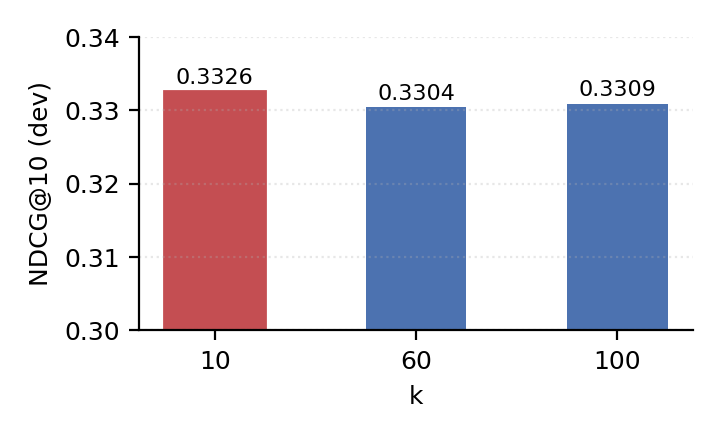
\includegraphics[width=.8\linewidth]{fig_rrf_k.png}
    \caption{$\ndcg{}@10$ no \emph{dev} para cada valor de $k$ do \rrf{}.}
    \label{fig:rrfk}
\end{figure}

O ajuste de $k$ no \emph{dev} (Tabela~\ref{tab:rrfk}) selecionou $k=10$. Com esse valor, a fusão
melhora o recuperador inicial: o $\ndcg{}@10$ sobe de $0{,}3302$ (lexical) e $0{,}3160$
(semântico) para $0{,}3562$, e $\mathrm{P@10}$ e $\mathrm{R@10}$ também aumentam
(Tabela~\ref{tab:metricas}). O ganho é coerente com o papel complementar dos dois sistemas: o
\rrf{} combina a precisão do casamento lexical em termos técnicos com a cobertura semântica em
consultas com variação de vocabulário, sem comparar diretamente scores de escalas distintas.

\subsection{Reranking}
O reranking praticamente não alterou o $\ndcg{}@10$ global ($0{,}3562$ em ambos) e reduziu
levemente o $\mathrm{P@10}$ ($0{,}2601\to0{,}2508$), embora tenha elevado o $\map{}$
($0{,}1365\to0{,}1388$). A média, porém, esconde ganhos e perdas por consulta. Os dois maiores
ganhos foram \texttt{PLAIN-1320} (\emph{Harvard Physicians' Study II}, $\Delta\ndcg{}=+0{,}562$,
com o documento relevante MED-4929 subindo da posição 7 para a 2) e \texttt{PLAIN-541}
(\emph{American Dental Association}, $\Delta\ndcg{}=+0{,}297$). O caso de pouca alteração foi
\texttt{PLAIN-1008} (\emph{deafness}), uma consulta de termo raro em que o cross-encoder pouco
pôde reordenar. A piora ocorreu em \texttt{PLAIN-1679} (\emph{myelopathy}), $\Delta\ndcg{}=-0{,}387$,
em que o cross-encoder deslocou o relevante MED-1113 da posição 2 para a 9. O resultado indica
que o cross-encoder pequeno (\texttt{ms-marco}) ajuda em consultas em que o híbrido já traz
candidatos plausíveis mas mal ordenados, mas pode rebaixar documentos relevantes quando a
evidência lexical é fraca.

\subsection{Tempos}
A construção do índice levou $0{,}27$~s e a consulta lexical média, $0{,}40$~ms, confirmando a
eficiência do índice invertido (acesso apenas às \emph{posting lists} dos termos da consulta). A
geração dos $3\,633$ embeddings levou $116{,}2$~s ($\approx1{,}9$~min); com eles pré-computados, a
consulta semântica leva em média $13{,}79$~ms. O reranking foi a etapa mais
lenta ($4{,}2$~s por consulta em CPU), coerente com a passagem de 50 pares (consulta, documento)
pelo cross-encoder. Sob pressão de memória, esse tempo chegou a $\approx98$~s por consulta,
evidenciando a sensibilidade do ambiente a troca de memória (swapping).

\subsection{RAG}

\textbf{Recuperação do contexto.} Para as 10 consultas do experimento, o $\mathrm{Hit@5}$ foi
$9/10$ --- em 9 consultas ao menos um documento relevante chegou ao contexto da LLM. O
$\mathrm{Recall@5}$ médio foi $0{,}108$, baixo como esperado (as consultas do \textsc{NFCorpus}
têm em média $\approx38$ relevantes, e apenas 5 documentos são enviados).

\textbf{Avaliação da geração.} A Tabela~\ref{tab:rag} resume as notas humanas (0--2) por condição.

\begin{table}[h]
\centering
\small
\begin{tabular}{lcc}
\toprule
Critério & Sem RAG (A) & Com RAG (B)\\
\midrule
Fidelidade & 1{,}40 & \textbf{1{,}60}\\
Completude & \textbf{1{,}90} & 1{,}60\\
Utilidade & \textbf{1{,}80} & 1{,}50\\
Rastreabilidade & --- & \textbf{1{,}30}\\
\bottomrule
\end{tabular}
\caption{Médias das notas (0--2) nas duas condições. A rastreabilidade da condição A é N/A e
fica excluída da média.}
\label{tab:rag}
\end{table}

\begin{figure}[h]
    \centering
    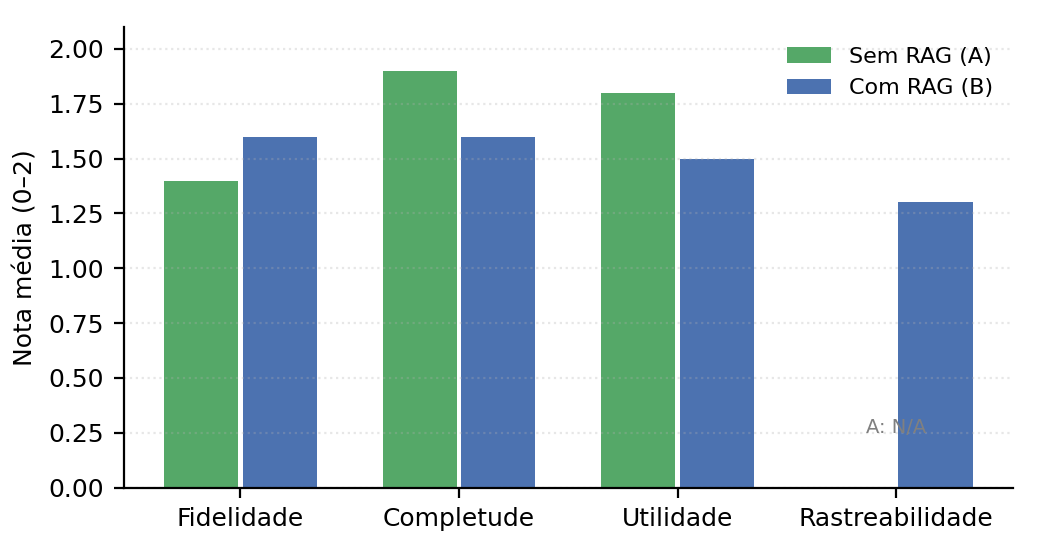
\includegraphics[width=.9\linewidth]{fig_rag_ab.png}
    \caption{Médias das notas humanas nas condições sem RAG (A) e com RAG (B).}
    \label{fig:rag}
\end{figure}

O RAG melhora a fidelidade ($1{,}40\to1{,}60$) e introduz rastreabilidade ($1{,}30$), enquanto a
condição sem RAG pontua mais em completude e utilidade ($1{,}90$ e $1{,}80$ contra $1{,}60$ e
$1{,}50$). Na condição A não há contexto externo fornecido à LLM (registrado explicitamente no
\texttt{rag\_experiment.csv}), e sua rastreabilidade é \texttt{N/A}, excluída da média. A fidelidade
da condição A foi avaliada comparando a resposta com os mesmos Top-5 documentos usados na condição B.
Essa aparente vantagem da condição A reflete o fato de as respostas sem RAG serem
fluentes e ``completas'', porém frequentemente alucinadas: sem acesso à coleção, a LLM inventa
conteúdo plausível mas sem suporte. As respostas com RAG, por outro lado, são mais curtas e
cautelosas --- às vezes declarando ausência de evidência --- o que reduz completude/utilidade,
mas ancora as afirmações no contexto e nas fontes. Isso ilustra exatamente o que o enunciado
aponta: o objetivo não é mostrar que o RAG sempre gera respostas melhores, mas investigar seu
efeito sobre qualidade, fidelidade e evidência.

\subsubsection{Análise de falhas ponta a ponta}
\begin{itemize}
  \item \textbf{RAG melhorou} --- \texttt{PLAIN-68} (\emph{What is Actually in Chicken Nuggets?}):
  a condição A afirmou que nuggets contêm ``frango processado, sal, açúcar, gelatina''
  (fidelidade $0$), contradizendo a evidência; a condição B respondeu ``nuggets são principalmente
  gordura'', citando o MED-2991 (fidelidade $2$).
  \item \textbf{Pouca diferença} --- \texttt{PLAIN-153} (\emph{How Should I Take Probiotics?}):
  as notas de qualidade foram idênticas ($2,2,2$), mudando apenas a rastreabilidade (a condição B
  cita a fonte).
  \item \textbf{RAG prejudicou} --- \texttt{PLAIN-238} (\emph{How Chemically Contaminated Are
  We?}): a condição A deu resposta coerente ($2,2,2$), enquanto a B ($1,1,0$) descreveu o documento
  MED-2391 sem responder à pergunta e ainda afirmou ``não posso afirmar quais doc\_ids foram
  usados'' --- embora os doc\_ids estivessem explicitamente no prompt. Investigando o estágio,
  constatamos que a recuperação funcionou (o MED-2391 relevante chegou ao contexto na posição 1);
  a falha foi na \emph{geração}, em que a LLM não sintetizou uma resposta direta apesar do contexto
  adequado.
\end{itemize}

%------------------------------------------------------------------------------
\section{Considerações Finais}
Os experimentos mostram que a busca lexical (\bmk{}) e a semântica (bi-encoder) têm desempenho
global próximo, com papéis complementares: o \bmk{} é superior em termos técnicos raros, o
bi-encoder em variação de vocabulário e sinonímia. A fusão por \rrf{} ($k=10$) aproveita essa
complementaridade e produz o melhor $\ndcg{}@10$ ($0{,}3562$). O reranking com cross-encoder
pequeno não alterou a média, mas gerou ganhos e perdas relevantes por consulta. A correção
ortográfica recuperou $6/7$ das consultas degradadas, falhando apenas em uma sigla rara ambígua.
O RAG elevou a fidelidade e a rastreabilidade das respostas, embora tenha reduzido completude e
utilidade ao evitar alucinações. Em suma, a combinação híbrida foi a escolha mais robusta, e a
análise por consulta revelou as limitações de cada componente --- especialmente a sensibilidade do
bi-encoder a termos de baixa frequência e a dependência da geração à capacidade da LLM de
sintetizar o contexto fornecido.

%------------------------------------------------------------------------------
\section{Uso de Ferramentas de IA}
Foram utilizadas ferramentas de IA generativa como apoio ao desenvolvimento: implementação e
depuração de código, estruturação do projeto e revisão textual deste relatório. Os modelos de
embeddings, o cross-encoder e a LLM (Qwen) são componentes do próprio experimento e estão
documentados na Metodologia, não constituindo uso de IA como ferramenta de apoio.

\end{document}
